\chapter{에너지, 운동량, 그리고 전자기장}

마지막 강의는 바로잡을 사항으로 시작해 아인슈타인 방정식의 우변에 놓일 대상으로 끝난다. 이 과정은 곁길로 빠지는 것이 아니다. 먼저 전기장의 부호 규약을 명확히 해야 하고, 이어 운동량의 서로 다른 세 가지 의미를 구분해야 한다. 이런 준비를 마친 뒤에야 장 이론을 공간의 각 점마다 자유도가 하나씩 있는 보통의 역학으로 읽을 수 있다. 그러면 해밀토니안, 국소 에너지 밀도, 뇌터 운동량, 전자기 에너지, 포인팅 벡터가 하나의 연속된 논증에서 차례로 도출된다.

\section{일관되게 유지해야 하는 부호 규약}

예비 노트를 수강생들에게 게시하기로 했지만, 이 문제는 강의 중에 직접 정리할 만큼 중요하다. Byron은 강의의 표기법 내부에 모순이 있는 것이 아니라, 그 표기법이 거의 모든 다른 곳에서 쓰이는 표기법과 일치하지 않는다는 점을 알아차렸다. 방정식을 매번 처음부터 유도할 때 생기는 직업상의 위험이다. 내부적으로는 일관된 사적 규약이 통용되는 표기법과 어긋날 수 있다.

표준 Maxwell--Franklin 규약에는 \(\mathbf E_M\)를, 앞선 강의에서 사용한 규약에는 \(\mathbf E_L\)를 쓰자. 강의의 공변 성분 \(A_0\)을 사용하면 두 규약은 다음과 같다.
\begin{align}
\mathbf E_M
  &= -\dot{\mathbf A}+\boldsymbol{\nabla}A_0,
&
\mathbf E_L
  &= +\dot{\mathbf A}-\boldsymbol{\nabla}A_0
   =-\mathbf E_M .
\label{eq:two-electric-conventions}
\end{align}많은 책에서는 대신 스칼라 퍼텐셜 \(\Phi=-A_0\)를 도입한다. 그러면 첫 번째 식은 다음과 같이 된다.
\(\mathbf E_M=-\dot{\mathbf A}-\boldsymbol{\nabla}\Phi\)
자기장은 바뀌지 않는다.
\begin{equation}
\mathbf B=\boldsymbol{\nabla}\times\mathbf A.
\label{eq:B-from-A-opening}
\end{equation}

\(c=1\)인 유리화 단위계에서 표준 Maxwell--Franklin 방정식은 다음과 같다.
\begin{align}
\boldsymbol{\nabla}\times\mathbf E_M&=-\dot{\mathbf B},
&
\boldsymbol{\nabla}\cdot\mathbf B&=0,
\nonumber\\
\boldsymbol{\nabla}\times\mathbf B&=\dot{\mathbf E}_M+\mathbf J_F,
&
\boldsymbol{\nabla}\cdot\mathbf E_M&=\rho_F .
\label{eq:maxwell-franklin}
\end{align}
Benjamin Franklin이 역사적으로 선택한 규약은 전하의 부호를 정한다. 이 규약에서 전자는 음전하를 띤다. 강의의 규약에서는 전하원의 표기도 반대로 바뀐다.
\begin{equation}
\mathbf J_L=-\mathbf J_F,
\qquad
\rho_L=-\rho_F.
\label{eq:source-convention-map}
\end{equation}
\(\mathbf E_L=-\mathbf E_M\)을 대입하면 다음을 얻는다.
\begin{align}
\boldsymbol{\nabla}\times\mathbf E_L&=+\dot{\mathbf B},
&
\boldsymbol{\nabla}\cdot\mathbf B&=0,
\nonumber\\
\boldsymbol{\nabla}\times\mathbf B&=-\dot{\mathbf E}_L-\mathbf J_L,
&
\boldsymbol{\nabla}\cdot\mathbf E_L&=\rho_L .
\label{eq:maxwell-course-convention}
\end{align}

\begin{figure}[H]\centering

\includegraphics[width=\linewidth]{lecture_10_figure_01.png}\caption{Maxwell--Franklin 규약과 강의 규약을 칠판에 모두 비교한 내용.}\par\smallskip
\textit{강의 영상 시각: 00:07:10.}\end{figure}

어느 표기법을 택하느냐에 따라 측정 가능한 결과가 달라지지는 않는다. 중요한 것은 일관성이다. 특히 계산한 장을 발표된 실험값과 비교할 때는 더욱 그렇다. 아이러니하게도 강연자의 연구에서는 이런 직접적인 수치 비교를 할 일이 거의 없었던 탓에, 반대 부호가 강의에서 지적될 때까지 눈에 띄지 않았다. 이 장의 뒤쪽에서 전자기장을 계산할 때는 표준 장 \(\mathbf E\equiv\mathbf E_M\)을 사용하겠다.

\section{운동량이라 불리는 서로 다른 세 가지 양}

이제 \emph{운동량}이라는 말을 풀어 구분해야 한다. 역학적 운동량, 정준 운동량, 뇌터 운동량은 간단한 문제에서는 서로 같을 수 있지만, 한 양을 달리 표현한 세 가지 방식은 아니다. 일반적인 계에서는 이들의 수치가 서로 다를 수 있다.

\subsection{역학적 운동량}

전체 질량이 \(M\)인 물체의 역학적 운동량은 다음과 같다.
\begin{equation}
\mathbf P_{\mathrm{mech}}=M\dot{\mathbf X}_{\mathrm{cm}}.
\label{eq:mechanical-momentum}
\end{equation}
입자 하나의 경우 \(\mathbf X_{\mathrm{cm}}\)는 단순히 그 입자의 위치다. 복합 물체에서는 질량중심이라는 한정이 필수적이다.

\begin{figure}[H]\centering
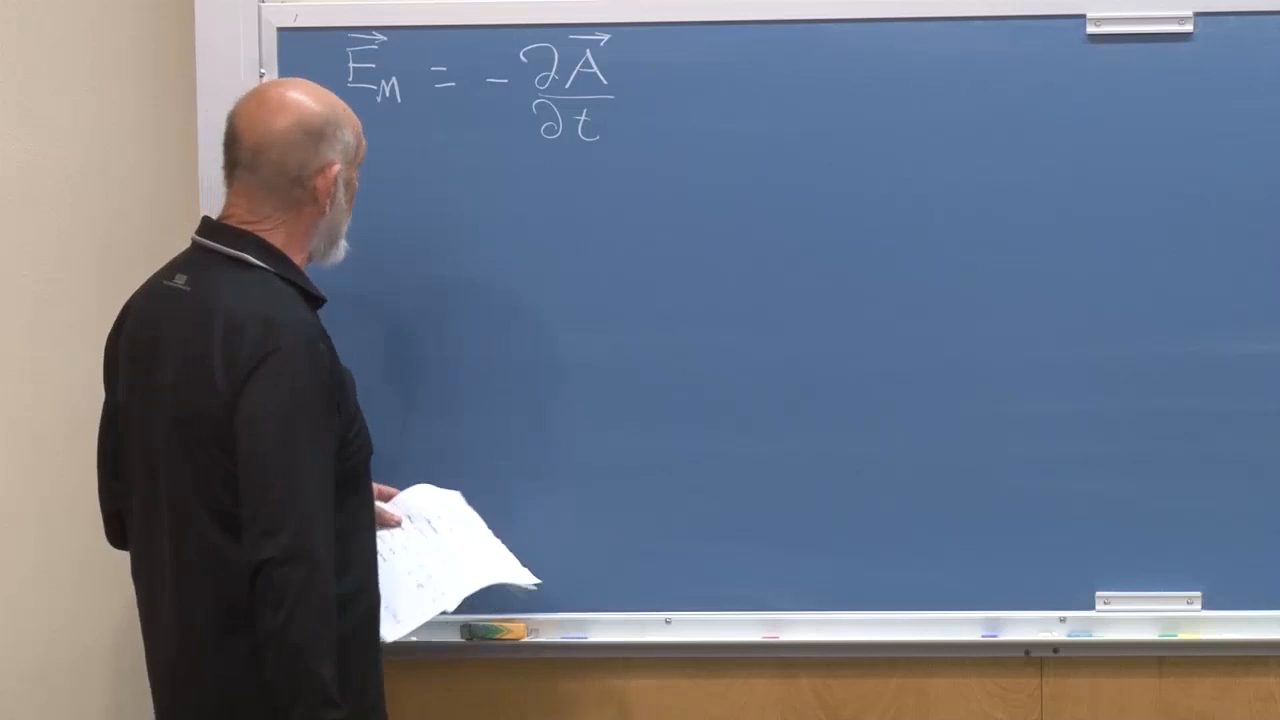
\includegraphics[width=\linewidth]{lecture_10_figure_02.png}\caption{역학적 운동량을 질량과 질량중심 속도의 곱으로 정의한다.}\par\smallskip
\textit{강의 영상 시각: 00:11:15.}\end{figure}

\subsection{정준 운동량}

역학이 다음과 같이 기술된다고 하자.
\(L(q_i,\dot q_i)\). \(q_i\)에 켤레인 정준 운동량은 다음과 같다.
\begin{equation}
p_i=\frac{\partial L}{\partial\dot q_i}.
\label{eq:canonical-momentum}
\end{equation}
\begin{equation}
L=\frac12 m\dot{\mathbf x}^{\,2}-V(\mathbf x),
\label{eq:simple-particle-lagrangian}
\end{equation}의 경우에는 \(\mathbf p=m\dot{\mathbf x}\)이므로 정준 운동량과 역학적 운동량이 우연히 일치한다.

\begin{figure}[H]\centering
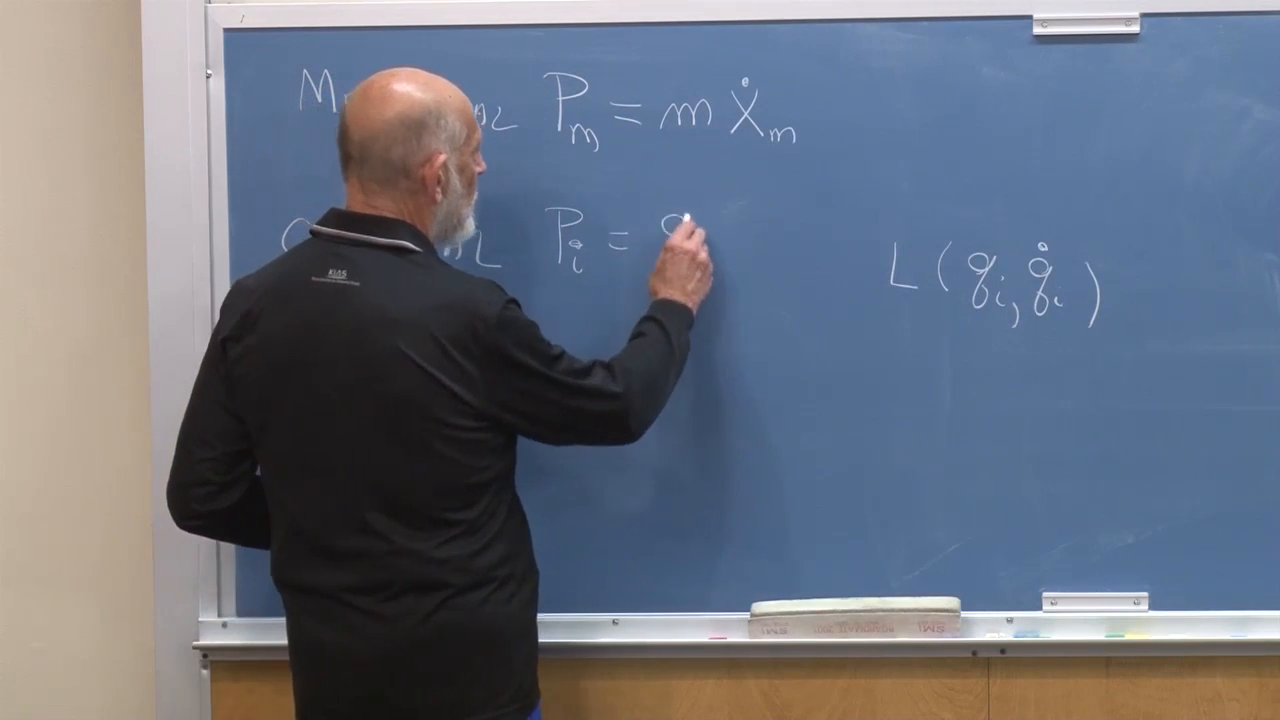
\includegraphics[width=\linewidth]{lecture_10_figure_03.png}\caption{단순한 입자 라그랑지안과 나란히 나타낸 역학적 운동량과 정준 운동량.}\par\smallskip
\textit{강의 영상 시각: 00:13:40.}\end{figure}

자기장 속의 하전 입자는 유용한 반례다. 칠판에 적은 부호 규약을 따르면
\begin{equation}
L=\frac12m\dot{\mathbf x}^{\,2}-V(\mathbf x)
  -e\,\dot{\mathbf x}\cdot\mathbf A(\mathbf x),
\label{eq:magnetic-particle-lagrangian}
\end{equation}
따라서
\begin{equation}
p_i=m\dot x_i-eA_i.
\label{eq:magnetic-canonical-shift}
\end{equation}
전하 또는 상호작용 항의 규약을 바꾸면 식에 나타나는 부호는 달라지지만, 핵심은 같다. 정준 운동량에는 벡터 퍼텐셜의 기여가 들어가며, 단순히 \(m\dot x_i\)인 것은 아니다. 해밀턴 방정식은 정준 변수를 사용한다. 나중에 장에 의존하는 항을 방정식의 반대편으로 옮기면 뉴턴 역학처럼 보이는 가속도 식을 얻을 수 있지만, 그렇게 식을 정리해도 정의 자체는 바뀌지 않는다.

\begin{figure}[H]\centering
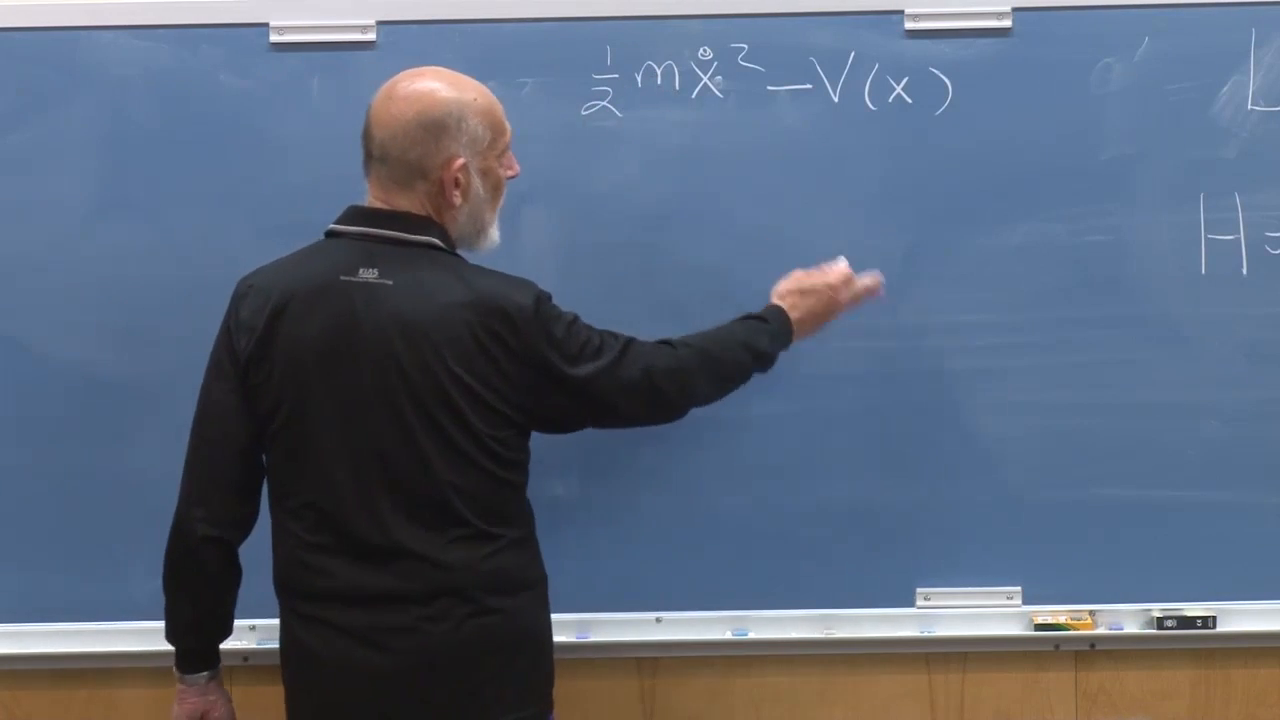
\includegraphics[width=\linewidth]{lecture_10_figure_04.png}\caption{벡터 퍼텐셜 항 때문에 정준 운동량은 역학적 운동량과 달라진다.}\par\smallskip
\textit{강의 영상 시각: 00:15:50.}\end{figure}

\subsection{뇌터 운동량}

세 번째 운동량은 공간 병진 대칭성에 대응하는 보존 전하다. 라그랑지안을 불변으로 두는 무한소 대칭 변환
\begin{equation}
q_i\longrightarrow q_i+\delta q_i
\end{equation}
에 대해 뇌터 정리는 무한소 매개변수의 정규화에 따라 다음을 준다.
\begin{equation}
Q=\sum_i p_i\,\delta q_i.
\label{eq:noether-charge-mechanics}
\end{equation}
여기에 나타나는 \(p_i\)는 정준 운동량이다. 대칭이 균일 병진이고 정준 운동량이 역학적 운동량과 우연히 같다면, \(Q\)는 익숙한 전체 운동량으로 환원된다. 더 복잡한 계에서는 그 일치를 가정하지 말고 증명해야 한다.

\begin{figure}[H]\centering
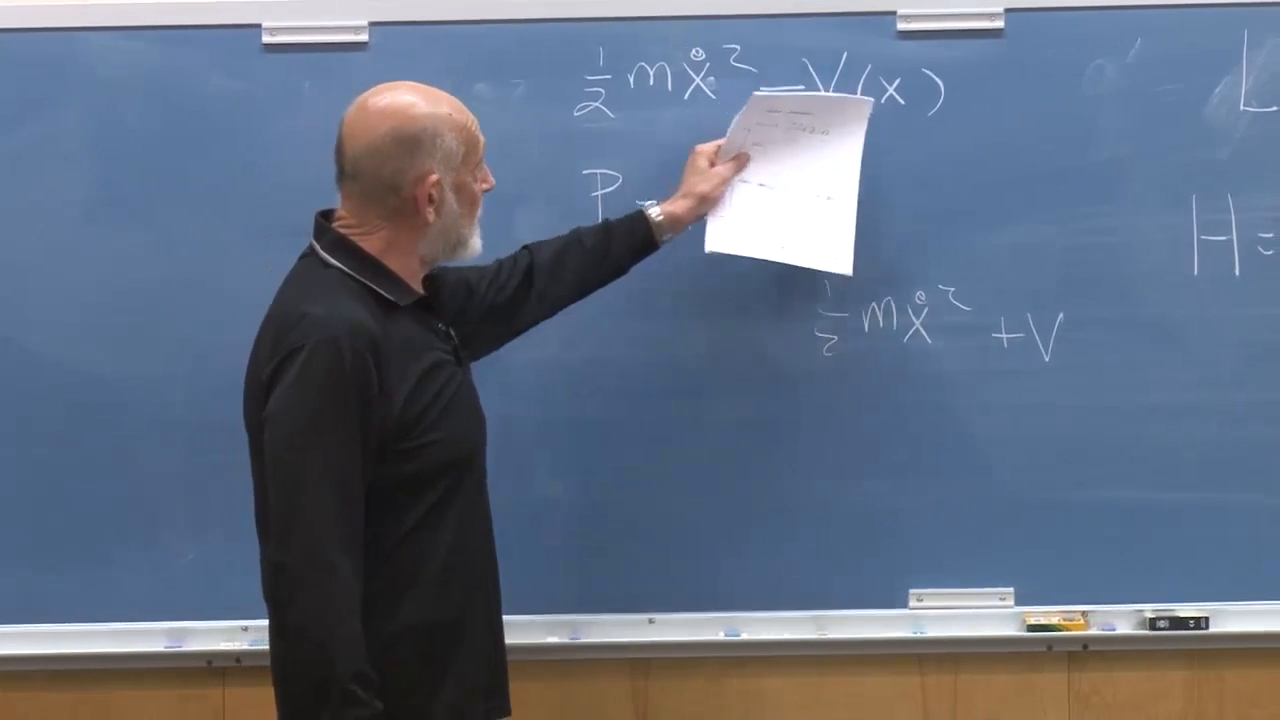
\includegraphics[width=\linewidth]{lecture_10_figure_05.png}\caption{정준 운동량과 좌표의 무한소 변화로 구성한 뇌터 전하.}\par\smallskip
\textit{강의 영상 시각: 00:19:00.}\end{figure}

\section{해밀토니안으로서의 에너지}

공간 병진은 운동량으로 이어지고, 시간 병진은 에너지로 이어진다. 라그랑지안이 시간에 명시적으로 의존하지 않으면 해밀토니안
\begin{equation}
H=\sum_i p_i\dot q_i-L
\label{eq:hamiltonian-definition}
\end{equation}
은 보존된다. 이것은 라그랑지안의 르장드르 변환이지, 식을 보고 부호를 바꾸는 규칙이 아니다.

\begin{figure}[H]\centering
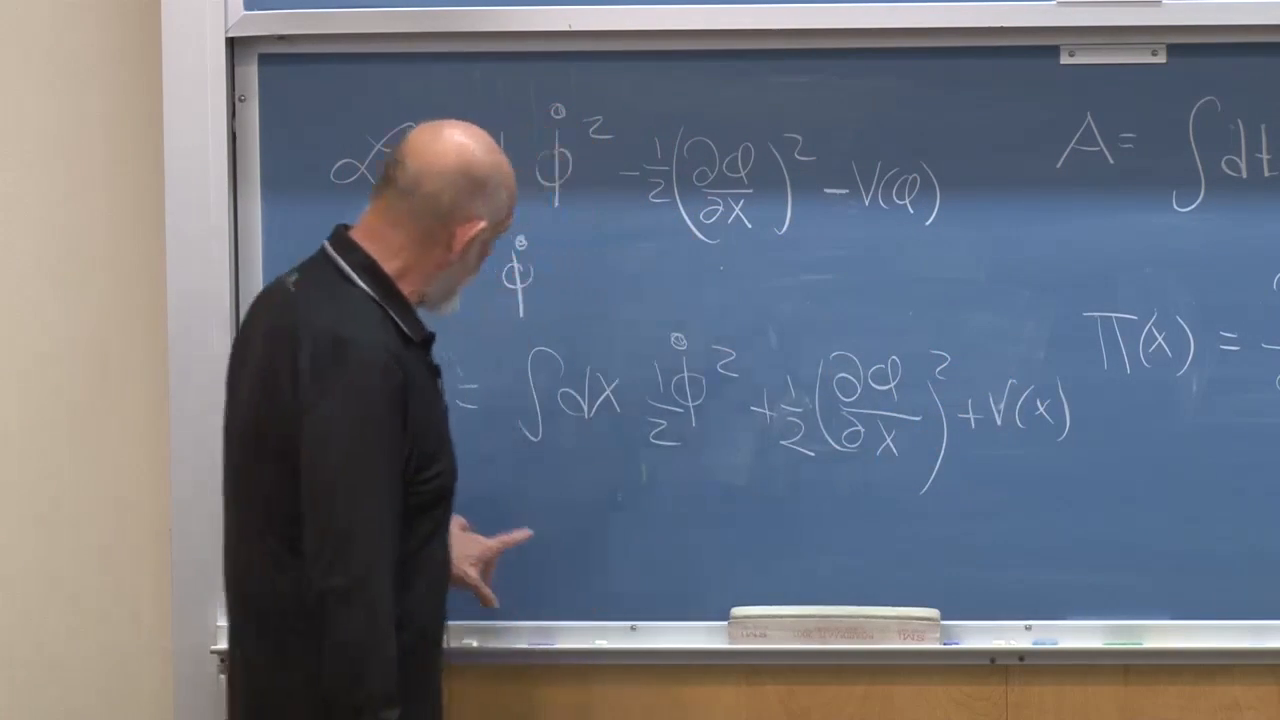
\includegraphics[width=\linewidth]{lecture_10_figure_06.png}\caption{일반적인 라그랑지안의 르장드르 변환으로 쓴 해밀토니안.}\par\smallskip
\textit{강의 영상 시각: 00:22:55.}\end{figure}

입자 하나의 예에서는
\begin{align}
p&=m\dot x,
\nonumber\\
H&=p\dot x-L\\
&=m\dot x^2
  -\left(\frac12m\dot x^2-V(x)\right)\\
&=\frac12m\dot x^2+V(x).
\label{eq:particle-hamiltonian}
\end{align}
따라서 라그랑지안은 운동에너지에서 퍼텐셜 에너지를 뺀 것이고, 해밀토니안은 운동에너지와 퍼텐셜 에너지를 더한 것이다.

\begin{figure}[H]\centering
\includegraphics[width=\linewidth]{lecture_10_figure_07.png}\caption{입자 계산을 통해 \(H=T+V\)가 \(H=p\dot x-L\)에서 어떻게 나오는지 보인다.}\par\smallskip
\textit{강의 영상 시각: 00:24:20.}\end{figure}

속도에 대한 모든 의존성이 표준적인 양의 이차 운동에너지 항이고 나머지 항에는 속도가 들어 있지 않다면, 속도가 없는 부분의 부호를 바꾸어 해밀토니안을 바로 읽어 낼 수 있다. 이 지름길은 앞으로 여러 번 쓰일 것이다. 여기서 다루는 예에서는 르장드르 변환이 이처럼 단순한 형태이므로 이 방법이 안전하다.

\section{장은 공간의 각 점에 연속적으로 무한히 많은 좌표가 있는 역학계다}

장 이론의 역학적 구조를 드러내기 위해 관성계를 하나 정하고, 잠시 각 식에 로런츠 공변성이 명시적으로 드러나야 한다는 요구를 내려놓자. 고전역학에는 시간축과 좌표 \(q_i(t)\)가 있다. 스칼라장에는 시간축과 좌표 \(\phi(\mathbf x,t)\)가 있다. 이산 표지 \(i\)가 연속 표지 \(\mathbf x\)로 바뀌었을 뿐이다.
\begin{equation}
q_i(t)\quad\longrightarrow\quad\phi(\mathbf x,t).
\label{eq:discrete-to-field}
\end{equation}
공간의 각 점에서 장이 갖는 값은 자유도 하나에 해당한다. 여기서 \(\mathbf x\)는 어떤 자유도를 가리키는 표지이지, 그 자체가 일반화 좌표는 아니다.

\begin{figure}[H]\centering
\includegraphics[width=\linewidth]{lecture_10_figure_08.png}\caption{공간 격자를 이용해 각 점의 장 값을 별도의 역학적 자유도로 나타낸 그림.}\par\smallskip
\textit{강의 영상 시각: 00:30:15.}\end{figure}

\begin{classroomqa}\audiencequestion{처음부터 장을 \(\phi(\mathbf x,t)\)라고 쓰면 안 되나요?}\lecturerresponse{그것이 완전한 표기법이다. 임시 표기 \(\phi(\mathbf x)\)는 흔히 \(q_i\)라고 쓰면서 각 \(q_i\)가 시간에 따라 변한다는 점을 염두에 두는 것처럼, 공통된 시간 인자를 생략한다. 표지 \(i\), 또는 이제는 \(\mathbf x\)가 논의 중인 자유도가 무엇인지 알려 준다. \lecturetimestamp{00:32:43}}\end{classroomqa}

\begin{classroomqa}\audiencequestion{서로 이웃한 점의 장 값은 정말 독립적인 좌표인가요? 연속성은 무엇이 보장하나요?}\lecturerresponse{이 값들은 독립적인 정준 좌표다. 이웃한 점들의 값을 서로 같게 두어 매끄러움을 강제하는 것은 아니다. 매끄러움은 동역학적으로 선택된다. 해밀토니안에는 양의 기울기 에너지 항이 있으므로, 거리가 점점 작아지는 두 점 사이에 고정된 불연속이 있으면 에너지 비용이 계속 커진다. 따라서 유한 에너지인 배치는 연속체 극한에서 매끄럽다. \lecturetimestamp{00:33:09}}\end{classroomqa}

공간 미분을 쓰면 이웃한 자유도 사이의 결합이 명시적으로 드러난다. 격자 간격이 \(\epsilon\)일 때,
\begin{equation}
\partial_x\phi(x,t)
  =\lim_{\epsilon\to0}
   \frac{\phi(x+\epsilon,t)-\phi(x,t)}{\epsilon}.
\label{eq:field-finite-difference}
\end{equation}
이 식은 서로 가까운 두 좌표에 의존하지만 일반화 속도는 포함하지 않는다. 역학적 비유에서 이것은 라그랑지안의 좌표 의존성에 해당하며 \(\dot q_i\) 의존성에는 해당하지 않는다.

\begin{figure}[H]\centering
\includegraphics[width=\linewidth]{lecture_10_figure_09.png}\caption{격자에서 이웃한 장 값의 차로 나타낸 공간 미분.}\par\smallskip
\textit{강의 영상 시각: 00:31:40.}\end{figure}

이제 작용을 명시적인 역학 형태로 쓸 수 있다.
\begin{align}
S&=\int dt\,L,
\nonumber\\
L&=\int d^3x\,
\mathcal L\!\left(
\phi,\dot\phi,\boldsymbol{\nabla}\phi
\right),
\nonumber\\
S&=\int dt\,d^3x\,
\mathcal L\!\left(
\phi,\dot\phi,\boldsymbol{\nabla}\phi
\right).
\label{eq:field-action-split}
\end{align}
필기체 문자 \(\mathcal L\)는 라그랑지안 밀도다. 이를 공간에 대해 적분하면 시간에 대해 다시 적분하는 보통의 라그랑지안을 얻는다. 국소 이론에서는 각 점의 장과 그 점에서의 미분을 통해서만 점들 사이에 결합이 생긴다. 시간과 공간을 분리하면 잠시 로런츠 공변성이 드러나지 않지만, 역학적 구조는 명확해진다.

\begin{figure}[H]\centering
\includegraphics[width=\linewidth]{lecture_10_figure_10.png}\caption{시간 적분과 라그랑지안 밀도의 공간 적분으로 나누어 쓴 장의 작용.}\par\smallskip
\textit{강의 영상 시각: 00:36:40.}\end{figure}

\section{정준 장 운동량과 해밀토니안 밀도}

장 좌표의 속도는 \(\dot\phi(\mathbf x,t)\)이다. 즉, 한 고정된 점에서 장이 시간에 따라 변하는 비율이다. 한 공간점에서 다른 공간점으로 이동하는 운동을 뜻하지 않는다. 따라서 장에 켤레인 정준 운동량 자체도 장이다.
\begin{equation}
\Pi(\mathbf x,t)
 =\frac{\partial\mathcal L}{\partial\dot\phi(\mathbf x,t)}.
\label{eq:field-canonical-momentum}
\end{equation}
여러 장 \(\phi_a\)이 있으면 각각에 대해 운동량 장 \(\Pi_a\)가 하나씩 있다.

르장드르 변환의 이산 합은 공간 적분으로 바뀐다.
\begin{align}
H
 &=\int d^3x\,
   \left[\Pi\dot\phi-\mathcal L\right]
  =\int d^3x\,\mathcal H,
\nonumber\\
\mathcal H
 &=\Pi\dot\phi-\mathcal L .
\label{eq:field-hamiltonian-density}
\end{align}
적분 안의 양이 에너지 밀도다.

\begin{figure}[H]\centering
\includegraphics[width=\linewidth]{lecture_10_figure_11.png}\caption{장에 대한 르장드르 변환과 이를 국소 에너지 밀도의 적분으로 해석한 식.}\par\smallskip
\textit{강의 영상 시각: 00:42:40.}\end{figure}

\begin{classroomqa}\audiencequestion{한 점에서 전체 라그랑지안을 \(\dot\phi\)에 대해 미분한 것을 그 점의 국소 밀도에 대한 미분으로 바꾸어도 되는 이유는 무엇인가요?}\lecturerresponse{공간 적분을 연속적인 합이라고 생각하면 된다. 여기서 가정한 국소성에 따르면 속도 \(\dot\phi(\mathbf x)\)는 바로 그 점에 해당하는 항에만 나타난다. 그 속도 하나에 대해 미분하면 다른 모든 항은 사라진다. 공간 미분은 이웃한 장 값들을 결합할 수 있지만, 이 이론에서는 이웃한 점의 시간 미분을 끌어들이지 않는다. \lecturetimestamp{00:51:56}}\end{classroomqa}

\subsection{스칼라장}

공간 차원이 하나일 때 다음을 취하자.
\begin{equation}
\mathcal L
 =\frac12\dot\phi^2
  -\frac12(\partial_x\phi)^2
  -V(\phi).
\label{eq:scalar-field-lagrangian}
\end{equation}
이는 앞서 사용한 로런츠 스칼라를 공변성이 명시적으로 드러나지 않는 형태로 쓴 것이다. 시간 미분과 공간 미분 사이의 상대적인 마이너스 부호는 민코프스키 계량에서 나온다. 정준 운동량은
\begin{equation}
\Pi=\dot\phi,
\label{eq:scalar-pi}
\end{equation}
이고 해밀토니안은 다음과 같다.
\begin{equation}
H=\int dx\,
\left[
\frac12\dot\phi^2
+\frac12(\partial_x\phi)^2
+V(\phi)
\right].
\label{eq:scalar-field-hamiltonian}
\end{equation}
계산 도중 퍼텐셜을 잠시 \(V(x)\)라고 불렀다가 수강생들이 \(V(\phi)\)로 바로잡았다. 장을 통해 간접적으로 위치에 의존할 수는 있지만, 병진 불변인 이론에서는 지정된 외부 \(x\) 의존성이 없다.

\begin{figure}[H]\centering
\includegraphics[width=\linewidth]{lecture_10_figure_12.png}\caption{스칼라 라그랑지안 밀도, 켤레 운동량, 양의 해밀토니안을 한 칠판에 모아 쓴 모습.}\par\smallskip
\textit{강의 영상 시각: 00:47:05.}\end{figure}

시간 미분이 전혀 없는 부분 전체가 퍼텐셜 에너지 역할을 한다. 여기에는 \(V(\phi)\)와 기울기 에너지 \(\frac12(\partial_x\phi)^2\)가 모두 포함된다. 라그랑지안은 어느 부호를 가져도 되지만, 안정한 에너지는 아래로 유계여야 한다.

\begin{classroomqa}\audiencequestion{\(V(\phi)\)는 음수일 수 있나요?}\lecturerresponse{그렇다. 유한한 하한이 있다면 상수를 더해 고전적 장 방정식을 바꾸지 않고도 최솟값을 0으로 만들 수 있다. 아래로 유계가 아닌 퍼텐셜은 불안정성을 뜻한다. 장의 에너지를 한계 없이 낮출 수 있기 때문이다. 안정한 진공은 상수인 장이 이동된 퍼텐셜의 최솟값에 놓인 상태다. \lecturetimestamp{00:49:03}}\end{classroomqa}

앞서 던진 연속성 질문에 이제 정량적으로 답할 수 있다. 격자 간격 \(\epsilon\)을 사이에 둔 불연속 \(\Delta\phi\)은 다음 기여를 한다.
\begin{equation}
\frac12(\partial_x\phi)^2
\sim\frac12\left(\frac{\Delta\phi}{\epsilon}\right)^2.
\label{eq:gradient-cost}
\end{equation}
\(\epsilon\to0\)일 때 고정된 불연속은 임의로 큰 에너지 밀도를 만든다. 따라서 유한 에너지는 들쭉날쭉한 배치를 억제한다.

\begin{figure}[H]\centering
\includegraphics[width=\linewidth]{lecture_10_figure_13.png}\caption{칠판 그림에서 매끄러운 장과 급격한 변화를 대비하며 유지한 스칼라 에너지 식.}\par\smallskip
\textit{강의 영상 시각: 00:54:20.}\end{figure}

\section{국소 에너지와 \texorpdfstring{\(T^{00}\)}{00}의 의미}

에너지 밀도에는 간결한 이름이 붙어 있다.
\begin{equation}
T^{00}=\mathcal H=\Pi\dot\phi-\mathcal L.
\label{eq:T00-definition}
\end{equation}
위첨자 0이 두 개 붙은 것은 서로 별개의 두 가지 진술을 나타낸다. 에너지는 에너지--운동량 사벡터의 시간 성분 \(P^0\)이고, 밀도는 보존 전류의 시간 성분이다. 따라서 \(T^{00}\)는 사차원 운동량의 시간 성분 밀도다.

\begin{figure}[H]\centering
\includegraphics[width=\linewidth]{lecture_10_figure_14.png}\caption{국소적으로 나타내고 \(T^{00}\)와 동일시한 장의 에너지.}\par\smallskip
\textit{강의 영상 시각: 01:00:00.}\end{figure}

상대론적 국소 이론에서 보존은 하나의 전역적인 수가 변하지 않는다는 말에 그치지 않는다. 에너지가 실험실에서 사라졌다가 알파 센타우리에서 다시 나타날 수는 없다. 어떤 영역 안에서 일어난 변화는 그 경계를 통과하는 플럭스로 설명되어야 한다. 국소 형태로 쓰면
\begin{equation}
\partial_\mu T^{\mu\nu}=0,
\label{eq:stress-energy-continuity}
\end{equation}
첫 번째 첨자는 밀도 또는 플럭스의 방향을, 두 번째 첨자는 전달되는 성분 \(P^\nu\)을 나타낸다.

\begin{classroomqa}\audiencequestion{\(T^{00}\)를 밀도라고 부른다는 것은 전체 에너지를 이것의 적분으로 구한다는 뜻인가요?}\lecturerresponse{그렇다.
\(E=P^0=\int d^3x\,T^{00}\). 국소 밀도는 장에 대한 르장드르 변환의 적분함수다. 한 지점에서의 변화는 이웃한 지점들 사이를 흐르는 에너지 전류로 보상된다. \lecturetimestamp{00:59:06}}\end{classroomqa}

\section{공간 병진에서 나오는 운동량 밀도}

이제 이산 합을 공간 적분으로 바꾸어 뇌터 공식을 다시 보자. \(m\) 방향으로 작은 병진을 하면 수동적 규약에서 장은 다음과 같이 변한다.
\begin{equation}
\delta\phi
  =\phi(\mathbf x)-\phi(\mathbf x-\boldsymbol{\epsilon})
  =\epsilon^m\partial_m\phi+O(\epsilon^2),
\label{eq:translated-field-change}
\end{equation}
능동 병진과 수동 병진을 서로 바꾸면 전체 부호도 바뀐다. 이 규약을 정하면 물리적 생성자가 정해진다. \(\epsilon^m\)을 묶어 내면 뇌터 운동량은 다음 구조를 갖는다.
\begin{equation}
P_m\ \propto\ \int d^3x\,\Pi\,\partial_m\phi.
\label{eq:scalar-noether-momentum}
\end{equation}

\begin{figure}[H]\centering
\includegraphics[width=\linewidth]{lecture_10_figure_15.png}\caption{병진된 장 분포와 그 무한소 변화를 나타내는 미분.}\par\smallskip
\textit{강의 영상 시각: 01:04:20.}\end{figure}

\begin{classroomqa}\audiencequestion{무한소 병진량 \(\epsilon\)을 운동량 식에 남겨 두지 않은 이유는 무엇인가요?}\lecturerresponse{뇌터 전하는 먼저 \(\epsilon\)에 비례하는 형태로 얻어진다. 운동량은 임의의 병진 매개변수에 곱해지는 계수로 정의하므로, \(\epsilon\)로 나누어 없앤다. 보존량에 고정된 상수를 곱해도 보존 여부는 달라지지 않지만, 계수를 추출하면 표준 정규화를 얻는다. \lecturetimestamp{01:04:45}}\end{classroomqa}

\begin{classroomqa}\audiencequestion{연속체 적분에서 병진 간격이 \(dx\)가 되나요?}\lecturerresponse{두 양은 서로 다른 극한에서 나온다. 공간 표지로 붙은 자유도들의 합을 적분으로 바꿀 때 측도 \(dx\)가 생긴다. 병진 매개변수 \(\epsilon\)는 대칭 변환을 나타내며 뇌터 전하에서 인수로 묶어 낸다. 중간 단계의 추론에서 둘 다 무한소이지만, 역할은 서로 다르다. \lecturetimestamp{01:05:16}}\end{classroomqa}

강의의 표기법에서 운동량의 \(m\)성분 밀도는 다음과 같다.
\begin{equation}
T^{0m}=\Pi\,\partial_m\phi,
\label{eq:scalar-momentum-density}
\end{equation}
병진 부호 규약은 위와 같이 정했다. 스칼라 이론에서는 \(\Pi=\dot\phi\)이므로 이는 다음에 비례한다.
\(\dot\phi\,\partial_m\phi\).

\begin{figure}[H]\centering
\includegraphics[width=\linewidth]{lecture_10_figure_16.png}\caption{칠판에 쓴 뇌터 운동량 밀도 \(T^{0m}=\Pi\,\partial_m\phi\).}\par\smallskip
\textit{강의 영상 시각: 01:07:10.}\end{figure}

이는 파동이 실제로 운반하는 운동량이다. 병진 불변성은 장, 입자, 전하원, 장치를 모두 함께 병진할 때만 성립한다. 자유롭게 매달린 판이 광 펄스를 흡수하면 판은 반동을 받는다. 보통 빛에서는 효과가 아주 작지만, 충분히 강한 레이저는 작은 표적을 압축할 만큼 큰 운동량을 전달할 수 있다. 보존되는 전체 운동량은 입자와 장을 함께 포함한다.

\subsection{뉴턴 방정식에 해당하는 것은 무엇인가?}

식~\eqref{eq:scalar-field-lagrangian}에서 유도한 장의 오일러--라그랑주 방정식은 다음과 같다.
\begin{equation}
\ddot\phi-\nabla^2\phi=-\frac{dV}{d\phi}.
\label{eq:scalar-equation-of-motion}
\end{equation}
이는 장 이론에서 뉴턴 법칙에 해당한다.

\begin{figure}[H]\centering
\includegraphics[width=\linewidth]{lecture_10_figure_17.png}\caption{해밀토니안 및 운동량 밀도와 나란히 나타낸 스칼라장 방정식.}\par\smallskip
\textit{강의 영상 시각: 01:12:55.}\end{figure}

\begin{classroomqa}\audiencequestion{장에 대해 뉴턴 법칙에 해당하는 것은 무엇인가요?}\lecturerresponse{오일러--라그랑주 장 방정식이다. 여기서는 힘 항 \(-V'(\phi)\)가 있는 파동 방정식이다. \(m\ddot x=-V'(x)\)에 해당하는 역할은 다음이 한다.
\(\ddot\phi-\nabla^2\phi=-V'(\phi)\)
\lecturetimestamp{01:11:48}}\end{classroomqa}

\begin{classroomqa}\audiencequestion{제안된 장 라그랑지안이 옳은지는 어떻게 알 수 있나요? 장 방정식을 이미 알아야 하나요?}\lecturerresponse{어느 방향으로도 진행할 수 있다. 역사적으로는 뉴턴이나 맥스웰의 경우처럼 실험에서 방정식을 추론한 다음 작용을 찾을 수 있다. 현대 이론에서는 장의 종류, 국소성, 대칭성, 허용되는 소수의 항에서 출발해 방정식을 유도하고 예측을 검증하는 경우가 많다. 여기 적힌 스칼라장은 기본 장을 나타낼 수도 있지만, 구성 입자들에서 연속체 작용을 유도한 밧줄의 횡변위를 나타낼 수도 있다. \lecturetimestamp{01:12:55}}\end{classroomqa}

\section{시간 성분 게이지에서의 전자기장}

앞서 구한 성분 \(T^{00}\)와 \(T^{0m}\)는 에너지--운동량 텐서에 속한다. 나머지 성분은 에너지와 운동량의 플럭스를 나타낸다. 이 텐서는 나중에 중력의 원천이 되지만, 당장은 전자기장이 구체적인 예를 제공한다.

기본 전자기 좌표는 사중 퍼텐셜 \(A_\mu\)이다. 게이지 자유도에 따라 다음과 같이 변환할 수 있다:
\begin{equation}
A_\mu\longrightarrow A'_\mu=A_\mu+\partial_\mu S
\label{eq:gauge-transformation-lecture10}
\end{equation}
이때 \(F_{\mu\nu}\)는 변하지 않는다. \(S\)가 다음 조건을 만족하도록 택하자:
\begin{equation}
\partial_tS=-A_0.
\label{eq:temporal-gauge-choice}
\end{equation}
예를 들어, 각 공간 위치에서 \(A_0\)를 시간에 대해 적분할 수 있다. 그러면 변환된 시간 성분은 사라진다:
\begin{equation}
A'_0=A_0+\partial_tS=0.
\label{eq:temporal-gauge}
\end{equation}
이것이 시간 게이지다. 이 게이지를 택하면 \(A_0\)는 동역학적 좌표 목록에서 제외되지만, 가우스 법칙은 제약 조건으로 남고 시간에 무관한 잔여 게이지 자유도도 남는다.

\begin{figure}[H]\centering
\includegraphics[width=\linewidth]{lecture_10_figure_18.png}\caption{\(A_0=0\)이 되도록 \(\partial_tS=-A_0\)를 풀어 이용한 게이지 자유도.}\par\smallskip
\textit{강의 영상 시각: 01:20:15.}\end{figure}

이제부터 \(\mathbf E\)는 표준 Maxwell 전기장을 뜻한다고 하자. 게이지를 고정하기 전에는
\begin{equation}
E_m=-\partial_tA_m+\partial_mA_0,
\qquad
\mathbf B=\boldsymbol{\nabla}\times\mathbf A.
\label{eq:E-B-general-potential}
\end{equation}
시간 성분 게이지에서는 다음처럼 단순해진다.
\begin{equation}
\mathbf E=-\dot{\mathbf A},
\qquad
\mathbf B=\boldsymbol{\nabla}\times\mathbf A.
\label{eq:E-B-temporal-gauge}
\end{equation}
\(\mathbf A\)의 시간 미분은 전기장을, 공간 미분은 자기장을 만든다.

\begin{figure}[H]\centering
\includegraphics[width=\linewidth]{lecture_10_figure_19.png}\caption{시간 성분 게이지에서의 전기장과 자기장: \(\mathbf E=-\dot{\mathbf A}\) 및 \(\mathbf B=\nabla\times\mathbf A\).}\par\smallskip
\textit{강의 영상 시각: 01:23:50.}\end{figure}

\section{전자기 정준 운동량과 에너지}

자유 Maxwell 라그랑지안 밀도는 다음과 같다.
\begin{equation}
\mathcal L_{\mathrm{EM}}
 =-\frac14F_{\mu\nu}F^{\mu\nu}
 =\frac12\left(\mathbf E^2-\mathbf B^2\right).
\label{eq:maxwell-lagrangian-energy-lecture}
\end{equation}
시간 성분 게이지에서는
\begin{equation}
\mathcal L_{\mathrm{EM}}
 =\frac12\dot{\mathbf A}^{\,2}
  -\frac12(\boldsymbol{\nabla}\times\mathbf A)^2.
\label{eq:maxwell-lagrangian-temporal}
\end{equation}
스칼라장과 정확히 같은 형태다. 시간 미분의 제곱에서 공간 미분의 제곱을 뺀다.

\begin{figure}[H]\centering
\includegraphics[width=\linewidth]{lecture_10_figure_20.png}\caption{\(\mathbf A\)의 공간 성분에 대한 역학적 장 라그랑지안으로 다시 쓴 Maxwell 라그랑지안.}\par\smallskip
\textit{강의 영상 시각: 01:28:10.}\end{figure}

각 성분 \(A_m\)에는 정준 운동량이 하나씩 대응한다.
\begin{equation}
\Pi_m
 =\frac{\partial\mathcal L_{\mathrm{EM}}}
        {\partial\dot A_m}
 =\dot A_m
 =-E_m.
\label{eq:em-canonical-momentum}
\end{equation}
이는 규약이 중요한 이유를 구체적으로 보여 준다. 앞서 사용한 반대 전기장 규약에서는 마지막 식에 나타나는 부호가 바뀌지만, 정준 미분 자체는 바뀌지 않는다.

\begin{figure}[H]\centering
\includegraphics[width=\linewidth]{lecture_10_figure_21.png}\caption{\(A_x,A_y,A_z\)에 대응하는 세 운동량 장. 각각 해당 시간 미분과 같으며, 따라서 표준 전기장의 음수다.}\par\smallskip
\textit{강의 영상 시각: 01:30:20.}\end{figure}

이제 해밀토니안의 지름길을 정당화할 수 있다. 시간 미분이 없는 항의 부호를 바꾸면 된다. 전자기 에너지 밀도는
\begin{equation}
T^{00}_{\mathrm{EM}}
 =\mathcal H_{\mathrm{EM}}
 =\frac12\left(\mathbf E^2+\mathbf B^2\right),
\label{eq:em-energy-density}
\end{equation}
이고 전체 에너지는
\begin{equation}
H_{\mathrm{EM}}
 =\int d^3x\,
\frac12\left(\mathbf E^2+\mathbf B^2\right).
\label{eq:em-total-energy}
\end{equation}
이다. 라그랑지안 밀도와 달리 에너지 밀도는 음수가 될 수 없다.

\begin{figure}[H]\centering
\includegraphics[width=\linewidth]{lecture_10_figure_22.png}\caption{양의 값을 갖는 전자기 해밀토니안 밀도 \(\frac12(\mathbf E^2+\mathbf B^2)\).}\par\smallskip
\textit{강의 영상 시각: 01:32:00.}\end{figure}

진공 속 평면파에서는 \(\mathbf E\perp\mathbf B\)이고 두 장은 같은 위상으로 진동한다. \(c=1\)인 단위계에서는 두 장의 크기가 같다. 따라서 전기장과 자기장이 파동 에너지를 똑같이 나누어 가진다.
\begin{equation}
u_E=\frac12\mathbf E^2,
\qquad
u_B=\frac12\mathbf B^2,
\qquad
u_E=u_B.
\label{eq:plane-wave-energy-halves}
\end{equation}

\section{전자기 운동량의 유도}

이제 뇌터 병진 공식을 세 장 \(A_m\)에 대해 합산해야 한다. 물리적 운동량이 파동의 진행 방향을 향하도록 병진 부호를 정하면, \(n\)성분은 다음과 같다.
\begin{equation}
P_n
 =\int d^3x\,E_m\,\partial_nA_m,
\label{eq:em-canonical-noether-momentum}
\end{equation}
여기서 \(m\)에 대해 합한다. 강의에서는 부호 문제를 의도적으로 짚고 넘어간다. 부호는 앞서 정한 전기장 규약과 능동 또는 수동 병진의 선택에 달려 있다. 게이지 불변인 물리적 결과로 부호를 확정할 수 있다.

\begin{figure}[H]\centering
\includegraphics[width=\linewidth]{lecture_10_figure_23.png}\caption{세 성분의 벡터 퍼텐셜로 확장한 스칼라장 뇌터 공식.}\par\smallskip
\textit{강의 영상 시각: 01:36:40.}\end{figure}

적분함수에는 여전히 물리장만이 아니라 게이지 퍼텐셜이 들어 있다. \(E_m\partial_mA_n\)를 더하고 빼면
\begin{align}
E_m\partial_nA_m
 &=
 E_m\left(\partial_nA_m-\partial_mA_n\right)
 +E_m\partial_mA_n.
\label{eq:add-subtract-em-momentum}
\end{align}
첫 번째 항은 외적이다.
\begin{equation}
E_m\left(\partial_nA_m-\partial_mA_n\right)
  =(\mathbf E\times\mathbf B)_n.
\label{eq:cross-product-component}
\end{equation}
두 번째 항에는 부분적분을 적용한다.
\begin{align}
\int d^3x\,E_m\partial_mA_n
 &=
\int_{\partial V}d\Sigma_m\,E_mA_n
-\int d^3x\,A_n\partial_mE_m.
\label{eq:em-momentum-integration-parts}
\end{align}
장이 경계에서 충분히 빨리 감소해 경계항이 사라지고, 전하원이 없는 영역이라 \(\boldsymbol{\nabla}\cdot\mathbf E=0\)이면 두 번째 항은 기여하지 않는다.

\begin{figure}[H]\centering
\includegraphics[width=\linewidth]{lecture_10_figure_24.png}\caption{부분적분으로 더한 항을 \(\nabla\cdot\mathbf E\)로 옮긴 모습.}\par\smallskip
\textit{강의 영상 시각: 01:40:00.}\end{figure}

따라서 강의의 단위계에서 장의 전체 운동량은 다음과 같다.
\begin{equation}
\mathbf P_{\mathrm{EM}}
 =\int d^3x\,\mathbf E\times\mathbf B,
\qquad
\mathbf g_{\mathrm{EM}}
 =\mathbf E\times\mathbf B,
\label{eq:em-momentum-density}
\end{equation}
벡터 \(\mathbf g_{\mathrm{EM}}\)는 전자기 운동량 밀도다.

\begin{figure}[H]\centering
\includegraphics[width=\linewidth]{lecture_10_figure_25.png}\caption{게이지 퍼텐셜로 나타낸 식을 게이지 불변 운동량 \(\int d^3x\,\mathbf E\times\mathbf B\)로 정리했다.}\par\smallskip
\textit{강의 영상 시각: 01:41:10.}\end{figure}

\begin{classroomqa}\audiencequestion{어디에서 \(\boldsymbol{\nabla}\cdot\mathbf E=0\)를 사용했나요? 전하가 있으면 어떻게 되나요?}\lecturerresponse{부분적분 뒤에 남는 부피항을 없앨 때 사용했다. 따라서 위에서 제시한 장만을 다루는 유도는 자유 전자기파에 적용된다. 전하가 있으면 그 항은 0이 아니므로 하전 물질의 운동량도 포함해야 한다. 병진 불변성과 운동량 보존은 물질--장 전체 계에 관한 것이다. \lecturetimestamp{01:41:55}}\end{classroomqa}

\subsection{파동 운동량의 방향}

평면파에서 \(\mathbf E\), \(\mathbf B\), 진행 방향은 오른손 좌표계를 이룬다. 반 파장만큼 진행하면 \(\mathbf E\)와 \(\mathbf B\)가 모두 방향을 바꾼다.
\begin{equation}
(-\mathbf E)\times(-\mathbf B)
 =\mathbf E\times\mathbf B.
\label{eq:poynting-sign-reversal}
\end{equation}
따라서 운동량 밀도는 진동 내내 한 방향을 유지하며, 그 방향은 파동의 진행 방향이다.

\begin{figure}[H]\centering
\includegraphics[width=\linewidth]{lecture_10_figure_26.png}\caption{평면파의 기하: 전기장과 자기장은 함께 방향을 바꾸지만, 두 장의 외적은 계속 진행축을 향한다.}\par\smallskip
\textit{강의 영상 시각: 01:43:10.}\end{figure}

이 때문에 빛의 압력은 실제로 존재한다. 흡수되면 장의 운동량이 물질로 전달되고, 반사되면 빛의 운동량 방향이 뒤집혀 반사체에 법선 성분의 두 배까지 전달될 수 있다.

\section{퍼텐셜과 관측 가능한 장의 접점}

\(A_\mu\)와 관측 가능한 장이 만나는 접점은 어디일까? 수업을 마무리하며 학생들은 이 질문을 던진다. 그 접점은 바로 다음과 같다.
\begin{align}
E_n&=-\partial_tA_n+\partial_nA_0,
\nonumber\\
B_n&=\epsilon_{nmk}\partial_mA_k.
\label{eq:potential-field-contact}
\end{align}
시간 게이지를 택하면 \(A_0\) 항은 사라지지만 물리적 장은 바뀌지 않는다.

\begin{figure}[H]
\centering
\includegraphics[width=\linewidth]{lecture_10_figure_27.png}
\caption{시간 게이지에서 계산한 뒤 복원한 일반적인 전기장 관계식과, 그 아래에 다시 제시한 공변 스칼라 라그랑지안.}
\par\smallskip
\textit{강의 화면: 01:45:40.}
\end{figure}

\begin{classroomqa}
\audiencequestion{벡터 퍼텐셜과 전기장 및 자기장은 정확히 어떻게 연결되는가?}
\lecturerresponse{전기장은 공간 퍼텐셜의 시간 미분과 \(A_0\)의 공간 미분을 결합한 것이고, 자기장은 공간 퍼텐셜의 회전이다. 시간 게이지에서는 다음처럼 간단해진다.
\(\mathbf E=-\dot{\mathbf A}\) 그리고
\(\mathbf B=\nabla\times\mathbf A\).
\lecturetimestamp{01:44:15}}
\end{classroomqa}

\begin{classroomqa}
\audiencequestion{퍼텐셜은 \(\mathbf E\)와 \(\mathbf B\)보다 더 근본적인가?}
\lecturerresponse{작용과 게이지 원리는 \(A_\mu\)를 사용해 가장 자연스럽게 정식화되므로, 퍼텐셜은 구조적으로 근본적인 변수다. 그러나 \(A_\mu\)는 유일하지 않다. 게이지 변환으로 서로 연결된 퍼텐셜은 같은 물리를 나타내며, 국소 장은 게이지 불변이다. 두 진술은 서로 양립한다. 근본 변수라고 해서 반드시 직접 관측 가능해야 하는 것은 아니다. \lecturetimestamp{01:46:36}}
\end{classroomqa}

\begin{classroomqa}
\audiencequestion{게이지 퍼텐셜 자체가 힘을 가할 수 있는가?}
\lecturerresponse{게이지에 의존하는 표현으로부터 게이지에 의존하는 측정 가능 힘이 생길 수는 없다. 작용에서는 전하를 띤 물질이 퍼텐셜과 결합하지만, 고전적인 로런츠 힘은 게이지 불변인 전기장과 자기장만으로 완전히 쓸 수 있다.
\lecturetimestamp{01:47:49}}
\end{classroomqa}

\begin{classroomqa}
\audiencequestion{전기장과 자기장이 서로 교차하고 정적이라면,
그 운동량은 반드시 영이어야 하는가?}
\lecturerresponse{장 자체의 운동량은 반드시 영일 필요는 없다:
\(\mathbf E\times\mathbf B\)는 두 장이 모두 시간에 따라 변하지 않더라도 영이 아닐 수 있다. 닫힌 정적 장치에서 전체 운동량 수지에는 전하, 전류, 지지 구조물, 그리고 기계적 운동량이나 숨은 운동량도 포함된다. 전체 운동량이 균형을 이루어야 한다는 간단한 강의실 답변은 올바른 보존 법칙의 진술이다. 장의 기여분만 영이라고 두는 것은 지나치게 강한 주장이다.
\lecturetimestamp{01:48:01}}
\end{classroomqa}

\section{하나의 텐서, 포인팅 벡터의 두 가지 의미}

에너지--운동량 텐서는 모든 밀도와 플럭스를 한데 정리한다.
\begin{align}
T^{00}&=\text{energy density},\\
T^{0i}&=\text{\(i\)-momentum density},\\
T^{i0}&=\text{energy flux in the \(i\)-direction},\\
T^{ij}&=\text{\(j\)-momentum flux in the \(i\)-direction}.
\label{eq:stress-energy-components}
\end{align}
예를 들어 \(T^{31}\)는 단위 시간당 \(x\)-운동량이 \(z\) 방향을 법선으로 하는 단위 면적을 통과하는 양이다. 공간 성분 블록 \(T^{ij}\)은 응력 텐서다.

\begin{figure}[H]
\centering
\includegraphics[width=\linewidth]{lecture_10_figure_28.png}
\caption{칠판에는 밀도와 플럭스 성분이 에너지--운동량 텐서로 정리되기 시작한다.}
\par\smallskip
\textit{강의 화면: 01:51:10.}
\end{figure}

여기서 다루는 상대론적 계에서는 물리적인 에너지--운동량 텐서를 대칭으로 택할 수 있다.
\begin{equation}
T^{\mu\nu}=T^{\nu\mu}.
\label{eq:stress-energy-symmetry}
\end{equation}
따라서
\begin{equation}
T^{0i}=T^{i0}.
\label{eq:momentum-density-energy-flux}
\end{equation}
\(i\)-운동량의 밀도는 \(c=1\)일 때 \(i\) 방향의 에너지 플럭스와 같다. 이것이 청중의 마지막 질문, 곧 포인팅 벡터가 실제로 단위 면적당 전력인지에 대한 답이다.

\begin{classroomqa}
\audiencequestion{\(\mathbf E\times\mathbf B\)는 운동량 밀도가 아니라 전력 밀도인가?}
\lecturerresponse{둘 다다. \(T^{\mu\nu}\)의 대칭성에 따라 운동량 밀도 \(T^{0i}\)는 에너지 플럭스 \(T^{i0}\)와 같다. 그러므로 \(\mathbf S=\mathbf E\times\mathbf B\)는 단위 시간당 단위 면적을 통과하는 에너지이며, \(c=1\) 단위계에서는 단위 부피당 운동량이기도 하다. 통상적인 단위를 복원하면 \(\mathbf g=\mathbf S/c^2\).
\lecturetimestamp{01:48:20}}
\end{classroomqa}

\begin{figure}[H]
\centering
\includegraphics[width=\linewidth]{lecture_10_figure_29.png}
\caption{운동량 밀도와 에너지 플럭스를 같게 두는 대칭 텐서 관계를 칠판에 포인팅 벡터로 표시했다.}
\par\smallskip
\textit{강의 화면: 01:53:50.}
\end{figure}

\section{일반상대성이론으로 가는 다리}

강의는 고전역학, 장 이론, 전자기학을 하나의 구조로 엮으며 마무리된다.
\begin{enumerate}
\item 시간 병진 대칭성은 해밀토니안과 에너지를 준다.
\item 공간 병진 대칭성은 뇌터 운동량을 준다.
\item 이산적인 좌표를 공간상의 각 점에 붙은 장으로 바꾸면 합은 적분으로, 보존량은 국소 밀도로 바뀐다.
\item 게이지를 고정하면 관측량을 바꾸지 않은 채 맥스웰 장의 역학적 좌표를 드러낼 수 있다.
\item 맥스웰 해밀토니안은 다음을 주고,
\(\frac12(\mathbf E^2+\mathbf B^2)\) 공간 병진은 다음을 준다.
\(\mathbf E\times\mathbf B\).
\item 대칭 에너지--운동량 텐서는 에너지 밀도, 운동량 밀도, 에너지 플럭스, 응력을 하나로 통합한다.
\end{enumerate}

다음 단계에서 필요한 물리량이 바로 이것이다. 일반상대성이론에서 에너지--운동량 텐서는 아인슈타인 장방정식의 원천으로 나타난다. 따라서 마지막 강의는 전자기학 계산을 덧붙이는 데 그치지 않고, 물질과 장이 시공간에 어떻게 곡률을 부여하는지를 기술하는 언어를 마련했다.
